\section{Rocket-API Service}
\label{sec:komponenten:rocket-api-service}
Um Endnutzern nicht die Last von Kubernetes aufzuerlegen, dient der Rocket-API Service als Mittelschicht zwischen
Client und Kubernetes. Hierbei wurde mit Hilfe von Googles gRPC\footnote{\href{https://grpc.io/}{gRPC}} Framework
eine API konzipiert, welche Standard CRUD\footnote{Create, Read, Update, Delete} Operationen, sowie das Auslesen
von Containerlogs implementiert.
Anfragen an die API werden mittels OAuth2 Middleware überprüft, um Authentifizierung zu garantieren. Um sicherzustellen,
dass jeder Nutzer nur auf seine eigenen Services zugreifen kann, werden alle Anfragen an die Kubernetes API als der
Nutzer selbst gestellt. Dies wird durch die Verbindung von Kubernetes, Keycloak und dem Rocket API-Service möglich.
Jeder Client implementiert das OpenID Connect Protokoll, um den Nutzer an der Authentifizierungsstelle, dem Keycloak
Server, anzumelden. Das erhaltene OpenID Token wird als HTTP Header in jeder Anfrage an den Rocket API-Service 
mitgeliefert. Dargestellt ist dieser Ablauf in \ref{fig:rocket-api-service-flow}.

\begin{figure}[h]
  \centering
  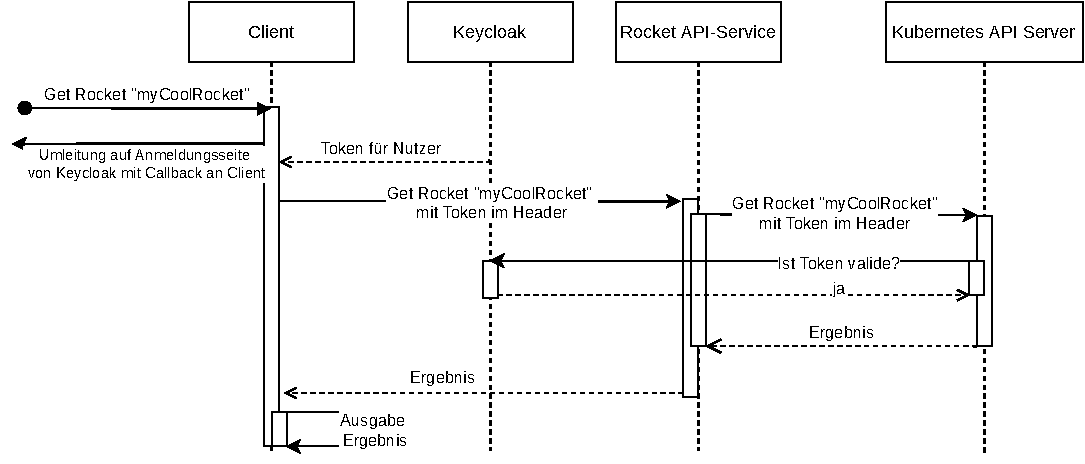
\includegraphics[height=0.5\textwidth]{gfx/chapters/3_komponenten/api-service-flow.pdf}
  \caption{Ablauf des Rocket API-Services}
  \label{fig:rocket-api-service-flow}
\end{figure}